\documentclass[tikz,border=0pt,tightpage]{standalone}
\usepackage{graphicx}
\usepackage{anyfontsize}
\usetikzlibrary{backgrounds}
\usetikzlibrary{calc}
\usepackage{tcolorbox}

\def\height{1}
\definecolor{offwhite}{HTML}{fbfbf9}
\definecolor{darkgray}{HTML}{b0b0b0}
\definecolor{lightgray}{HTML}{dedede}
\definecolor{dpurple}{HTML}{43204c}
\definecolor{lpurple}{HTML}{c9b5c8}
\definecolor{gre1}{HTML}{e1e9da}
\definecolor{gre2}{HTML}{d0ddc6}
\definecolor{gre3}{HTML}{9eb988}
\definecolor{gre4}{HTML}{4a6038}
\definecolor{gre5}{HTML}{61a32c}
\definecolor{re1}{HTML}{edd9da}
\definecolor{re2}{HTML}{e1c1c2}
\definecolor{re3}{HTML}{c58587}
\definecolor{blu2}{HTML}{e1e9f0}
\definecolor{blu3}{HTML}{ced4d9}

\renewcommand{\familydefault}{\sfdefault}

\newcommand{\boxword}[1]{%
    \tcbox[
        on line,
        boxrule=0pt,    % Removes the border
        colframe=white,
        colback=offwhite,
        boxsep=2pt, 
        left=1pt, right=1pt, top=0pt, bottom=0pt
    ]{\strut #1}%
}

\begin{document}
\begin{tikzpicture}[
    every node/.style={font=\fontsize{26}{30}\selectfont},
]

\def\sectionsep{15}

\def\totalheight{12cm}

\def\titleheight{13}
\def\contextheight{12.2}
\def\promptheight{5.6}
\def\responseheight{1.8}

\def\combinedheight{-5.5}
\def\seperatedheight{-9.5}

% SENTENCE EXAMPLE
\def\boxwidth{18cm}
\node[name=ex1, anchor=north west] at (0, 0) {%
\begin{tikzpicture}[
    background rectangle/.style={
        fill=white,
        rounded corners=5mm,
    }, 
    show background rectangle,
    inner frame sep=0.5cm,
]

\path (0,-\totalheight) rectangle (0,\totalheight);

\node[anchor=center, text=black, font=\Huge] at (5, \titleheight) {\textbf{(a) SENTIMENT ANALYSIS}};

\node[name=fullimage, anchor=north] at (5, \contextheight) {%
\begin{tikzpicture}[
    background rectangle/.style={
        fill=blu2,
        rounded corners=2mm,
    }, 
    show background rectangle,
    inner frame sep=0.3cm,
]
\path (0, -4.5) rectangle (0, 0.5);

\node[anchor=west, text=black, text width=\boxwidth, font=\rmfamily] at (0, 0.5) {\textbf{CONTEXT}};

\node[anchor=north west, text width=\boxwidth] 
at (0, 0) {
    \begin{minipage}{\boxwidth}
        \baselineskip=40pt
        ... \boxword{Her} \boxword{acting} \boxword{never} \boxword{fails} \boxword{to} \boxword{impress.} 
        \boxword{She} \boxword{brings} \boxword{depth} \boxword{and} \boxword{authenticity} \boxword{to} \boxword{every} \boxword{role.} 
        \boxword{Her} \boxword{performances} \boxword{consistently} \boxword{draw} \boxword{the} ...
    \end{minipage}
};




 


\end{tikzpicture}
};

\node[name=question, anchor=north] at (5, \promptheight) {%
\begin{tikzpicture}[
    background rectangle/.style={
        fill=blu2,
        rounded corners=2mm,
    }, 
    show background rectangle,
    inner frame sep=0.3cm,
]
\node[anchor=west, text=black, font=\rmfamily] at (0, 0) {\textbf{PROMPT}};
\node[anchor=north west, text width=\boxwidth, font=\fontsize{29}{30}\selectfont] at (0, -0.7) {\emph{Is this a positive or negative review?}};
\end{tikzpicture}
};

\node[name=answer, anchor=north] at (5, \responseheight) {%
\begin{tikzpicture}[
    background rectangle/.style={
        fill=blu3,
        rounded corners=2mm,
    }, 
    show background rectangle,
    inner frame sep=0.3cm,
]
\path (0, -3.3) rectangle (0, 0);
\node[anchor=west, text=black, font=\rmfamily] at (0, 0) {\textbf{GENERATED RESPONSE}};

\node[anchor=north west, text width=\boxwidth, font=\fontsize{29}{30}\selectfont] at (0, -1.2)
{\emph{Positive.}};

\end{tikzpicture}
};

%%% PATCHES

%%% Label
\node[anchor=west, text=black, font=\rmfamily] 
at (-4, \combinedheight) {\textbf{Interaction:}};

%%% First patch
\node[name=leftpatch, anchor=center, draw, rectangle, rounded corners, fill=re3, text=black, minimum width=2.5cm, minimum height=1.5cm, font=\Huge] 
at (3, \seperatedheight+1) {\strut never};

%%% Second patch
\node[name=rightpatch, anchor=center, draw, rectangle, rounded corners, fill=re3, text=black, minimum width=2.5cm, minimum height=1.5cm, font=\Huge] 
at (11, \seperatedheight+1) {\strut fails};

%%% combined patch
\node[name=combined, anchor=center] at (7, -4.5) {%
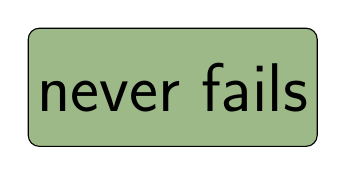
\begin{tikzpicture}

\node[draw, rectangle, rounded corners, fill=gre3, text=black, minimum width=2.5cm, minimum height=1.5cm, font=\Huge] 
at (0, 0) {never fails};

\end{tikzpicture}
};

\draw[-, line width = 1mm, black] (combined.south) + (-2, 0) -- (leftpatch.north) node[above] {};

\draw[-, line width = 1mm, black] (combined.south) + (2, 0) -- (rightpatch.north) node[above] {};


%%% First patch
\node[anchor=center, draw, rectangle, rounded corners, fill=gre1, text=black, minimum width=2.5cm, minimum height=1.5cm, font=\Huge] 
at (8.5, \seperatedheight - 2) {\strut never};

%%% Second patch
\node[anchor=center, draw, rectangle, rounded corners, fill=gre1, text=black, minimum width=2.5cm, minimum height=1.5cm, font=\Huge] 
at (12, \seperatedheight - 2) {\strut fails};

%%% Label
\node[anchor=west, text=black, font=\rmfamily] 
at (-4, \seperatedheight - 2) {\textbf{Marginal attributions:}};

\end{tikzpicture}
};

\draw[black] ([xshift=\sectionsep/2]ex1.north east) -- ++(0, - 27.5);

% DOCUMENT EXAMPLE
\def\boxwidth{28cm}
\node[name=ex2, anchor=north west] at ([xshift=\sectionsep]ex1.north east) {%
\begin{tikzpicture}[
    background rectangle/.style={
        fill=white,
        rounded corners=5mm,
    }, 
    show background rectangle,
    inner frame sep=0.5cm,
]

\path (0,-\totalheight) rectangle (1,\totalheight);

\node[anchor=center, text=black, font=\Huge] at (5, \titleheight) {\textbf{(b) RETRIEVAL AUGMENTED GENERATION}};

\node[name=fullimage, anchor=north] at (5, \contextheight) {%
\begin{tikzpicture}[
    background rectangle/.style={
        fill=blu2,
        rounded corners=2mm,
    }, 
    show background rectangle,
    inner frame sep=0.3cm,
]

\path (0, -2) rectangle (0, 2.5);

\node[anchor=center, text=black, text width=\boxwidth, font=\rmfamily] at (0, 3) {\textbf{CONTEXT}};

% \node[name=doc1, inner sep=3, anchor=west] at 
% (-6.5, 1.5) {
%     \includegraphics[width=2 cm]{figures/page.pdf}
% };
% \node[anchor=center, draw, rectangle, fill=white, text width=4.5cm, align=center] at ([yshift=-1cm]doc1.center) {Rio \;\;\;\;\;\;\;\;Carnival};

\node[name=doc6, inner sep=3, anchor=center, font=\fontsize{60}{50}\selectfont] at 
(-13.2, 0.3) {...};

\node[name=doc9, inner sep=3, anchor=west] at 
(-11.8, 0.3) {
    \includegraphics[width=1.4 cm]{figures/page.pdf}
};
\node[anchor=center, draw, rectangle, fill=offwhite, text width=1.8cm, align=center, rounded corners=2mm, font=, font=\fontsize{14}{14}\selectfont] at ([yshift=-0.6cm]doc9.center) {Weather in Tokyo};

\node[name=doc8, inner sep=3, anchor=west] at 
(-9.05, 0.5) {
    \includegraphics[width=1.7 cm]{figures/page.pdf}
};
\node[anchor=center, draw, rectangle, fill=offwhite, text width=2.5cm, align=center,rounded corners=2mm, font=\fontsize{20}{20}\selectfont] at ([yshift=-0.8cm]doc8.center) {Brazilian Music};

\node[name=doc2, inner sep=3, anchor=west] at 
(-5.5, 0.7) {
    \includegraphics[width=2 cm]{figures/page.pdf}
};
\node[anchor=center, draw, rectangle, fill=offwhite, text width=3.4cm, align=center, rounded corners=2mm] at ([yshift=-1cm]doc2.center) {Rio \;\;\;\;\;\;\;\;\;\;\;\;\;Carnival};

\node[name=doc3, inner sep=3, anchor=west] at 
(-1.3, 0.7) {
    \includegraphics[width=2 cm]{figures/page.pdf}
};
\node[anchor=center, draw, rectangle, fill=offwhite, text width=3.4cm, align=center, rounded corners=2mm] at ([yshift=-1cm]doc3.center) {Summer in Brazil};

\node[name=doc4, inner sep=3, anchor=west] at 
(2.9, 0.7) {
    \includegraphics[width=2 cm]{figures/page.pdf}
};
\node[anchor=center, draw, rectangle, fill=offwhite, text width=3.4cm, align=center, rounded corners=2mm] at ([yshift=-1cm]doc4.center) {Winter in Brazil
};

\node[name=doc8, inner sep=3, anchor=west] at 
(6.75, 0.5) {
    \includegraphics[width=1.7 cm]{figures/page.pdf}
};
\node[anchor=center, draw, rectangle, fill=offwhite, text width=2.5cm, align=center, rounded corners=2mm, font=\fontsize{20}{20}\selectfont] at ([yshift=-0.8cm]doc8.center) {History of Brazil};

\node[name=doc9, inner sep=3, anchor=west] at 
(9.8, 0.3) {
    \includegraphics[width=1.4 cm]{figures/page.pdf}
};
\node[anchor=center, draw, rectangle, fill=offwhite, text width=1.8cm, align=center, rounded corners=2mm, font=, font=\fontsize{14}{14}\selectfont] at ([yshift=-0.6cm]doc9.center) {Sport in Rio};

\node[name=doc6, inner sep=3, anchor=center, font=\fontsize{60}{50}\selectfont] at 
(12.9, 0.3) {...};

\end{tikzpicture}
};

\node[name=question, anchor=north] at (5, \promptheight) {%
\begin{tikzpicture}[
    background rectangle/.style={
        fill=blu2,
        rounded corners=2mm,
    }, 
    show background rectangle,
    inner frame sep=0.3cm,
]
\node[anchor=west, text=black, font=\rmfamily] at (0, 0) {\textbf{PROMPT}};
\node[anchor=north west, text width=\boxwidth, font=\fontsize{29}{30}\selectfont] at (0, -0.7){\emph{What is the weather like during Rio Carnival?}};
\end{tikzpicture}
};

\node[name=answer, anchor=north] at (5, \responseheight) {%
\begin{tikzpicture}[
    background rectangle/.style={
        fill=blu3,
        rounded corners=2mm,
    }, 
    show background rectangle,
    inner frame sep=0.3cm,
]
\path (0, -3.3) rectangle (0, 0);
\node[anchor=west, text=black, font=\rmfamily] at (0, 0) {\textbf{GENERATED RESPONSE}};
\node[anchor=north west, text width=\boxwidth, font=\fontsize{29}{30}\selectfont] at (0, -0.7){\emph{Rio Carnival generally takes place during the summer season in Brazil. The weather at this time is typically hot and humid.}};
\end{tikzpicture}
};

%%% PATCHES

%%% Label
\node[anchor=west, text=black, font=\rmfamily] 
at (-9.3, \combinedheight + 1) {\textbf{Interactions:}};

%%% First patch
\node[name=leftpatch, anchor=center] at (-3, \seperatedheight - 1) {%
\begin{tikzpicture}
\node[name=doc1, inner sep=3, anchor=center] at 
(1, 0) {
    \includegraphics[width=2 cm]{figures/page.pdf}
};
\node[anchor=center, draw, rectangle, fill=gre1, text width=3.5cm, align=center, rounded corners=2mm] at ([yshift=-1cm]doc1.center) {Summer in Brazil};
\end{tikzpicture}
};

%%% Second patch
\node[name=middlepatch, anchor=center] at (6, \seperatedheight - 1) {%
\begin{tikzpicture}
\node[name=doc1, inner sep=3, anchor=center] at 
(0, 0) {
    \includegraphics[width=2 cm]{figures/page.pdf}
};
\node[anchor=center, draw, rectangle, fill=gre1, text width=3.5cm, align=center, rounded corners=2mm] at ([yshift=-1cm]doc1.center) {Rio \;\;\;\;\;\;\;\;Carnival};
\end{tikzpicture}
};

%%% Third patch
\node[name=rightpatch, anchor=center] at (15, \seperatedheight - 1) {%
\begin{tikzpicture}
\node[name=doc1, inner sep=3, anchor=center] at 
(0, 0) {
    \includegraphics[width=2 cm]{figures/page.pdf}
};
\node[anchor=center, draw, rectangle, fill=re2, text width=4.5cm, align=center, rounded corners=2mm] at ([yshift=-1cm]doc1.center) {Winter in Brazil};
\end{tikzpicture}
};

%%% combined patch
\node[name=combined, anchor=center] at (1.5, \combinedheight) {%
\begin{tikzpicture}
\node[name=doc1, inner sep=3, anchor=center] at 
(-0.3, 0.4) {
    \includegraphics[width=2 cm]{figures/page.pdf}
};
\node[name=doc2, inner sep=3, anchor=center] at 
(0.3, 0) {
    \includegraphics[width=2 cm]{figures/page.pdf}
};
\node[anchor=center, draw, rectangle, fill=gre3, text width=7.5cm, align=center, rounded corners=2mm] at ([yshift=-1cm]doc2.center) {Rio Carnival \&\;\; Summer in Brazil};
\end{tikzpicture}
};

%%% second combined patch
\node[name=combined2, anchor=center] at (10.5, \combinedheight) {%
\begin{tikzpicture}
\node[name=doc1, inner sep=3, anchor=center] at 
(-0.3, 0.4) {
    \includegraphics[width=2 cm]{figures/page.pdf}
};
\node[name=doc2, inner sep=3, anchor=center] at 
(0.3, 0) {
    \includegraphics[width=2 cm]{figures/page.pdf}
};
\node[anchor=center, draw, rectangle, fill=re1, text width=7.5cm, align=center, rounded corners=2mm] at ([yshift=-1cm]doc2.center) {Rio Carnival \&\; Winter in Brazil};
\end{tikzpicture}
};

\draw[-, line width=1mm, black] ($(combined.south) + (-1, 0)$) -- ($(leftpatch.north) + (1.5, -1.2)$) node[above] {};

\draw[-, line width=1mm, black] ($(combined.south) + (1, 0)$) -- ($(middlepatch.north) + (-1.5, -1.2)$) node[above] {};

\draw[-, line width=1mm, black] ($(combined2.south) + (-1, 0)$) -- ($(middlepatch.north) + (1.5, -1.2)$) node[above] {};

\draw[-, line width=1mm, black] ($(combined2.south) + (1, 0)$) -- ($(rightpatch.north) + (-1.5, -1.2)$) node[above] {};

\end{tikzpicture}
};

\draw[black] ([xshift=\sectionsep/2]ex2.north east) -- ++(0, - 27.5);

% VQA EXAMPLE
\def\boxwidth{18cm}
\node[name=ex3, anchor=north west] at ([xshift=\sectionsep]ex2.north east) {%
\begin{tikzpicture}[
    background rectangle/.style={
        fill=white,
        rounded corners=5mm,
    }, 
    show background rectangle,
    inner frame sep=0.5cm,
]

\path (0,-\totalheight) rectangle (0,\totalheight);

\node[anchor=center, text=black, font=\Huge] at (5, \titleheight) {\textbf{(c) VISUAL QUESTION ANSWERING}};

\def\imageloc{figures/interaction_diagram/dog-3.png}

% Define the width and height of the image
\def\imagewidth{8.88} % Width of the image in cm
\def\imageheight{5} % Height of the image in cm

% Define the grid size and separation
\def\rows{2} % Number of rows
\def\cols{3} % Number of columns

 % Calculate patch dimensions
\pgfmathsetmacro{\patchwidth}{\imagewidth / \cols}
\pgfmathsetmacro{\patchheight}{(\imageheight / \rows}

\node[name=fullimage, anchor=north] at (5, \contextheight) {%
\begin{tikzpicture}[
    background rectangle/.style={
        fill=blu2,
        rounded corners=2mm,
    }, 
    show background rectangle,
    inner frame sep=0.3cm,
]

\node[anchor=center, text=black, text width=\boxwidth, font=\rmfamily] at (0, 0.5) {\textbf{CONTEXT}};

\node[anchor=north] at (2, 1.3) {\begin{tikzpicture}
\node[inner sep=0, anchor=south west] at 
(0, 0) {
    \includegraphics[width=\imagewidth cm, height=\imageheight cm]{\imageloc}
};
\draw[white, line width=2pt] (0, 0) rectangle ++(\patchwidth, \patchheight);
\draw[white, line width=2pt] (\patchwidth, 0) rectangle ++(\patchwidth, \patchheight);
\draw[white, line width=2pt] (2*\patchwidth, 0) rectangle ++(\patchwidth, \patchheight);
\draw[white, line width=2pt] (0, \patchheight) rectangle ++(\patchwidth, \patchheight);
\draw[white, line width=2pt] (\patchwidth, \patchheight) rectangle ++(\patchwidth, \patchheight);
\draw[white, line width=2pt] (2*\patchwidth, \patchheight) rectangle ++(\patchwidth, \patchheight);
\end{tikzpicture}
};

\end{tikzpicture}
};

\node[name=question, anchor=north] at (5, \promptheight) {%
\begin{tikzpicture}[
    background rectangle/.style={
        fill=blu2,
        rounded corners=2mm,
    }, 
    show background rectangle,
    inner frame sep=0.3cm,
]
\node[anchor=west, text=black, font=\rmfamily] at (0, 0) {\textbf{PROMPT}};
\node[anchor=north west, text width=\boxwidth, font=\fontsize{29}{30}\selectfont] at (0, -0.7){\emph{What is shown in this image?}};
\end{tikzpicture}
};

\node[name=answer, anchor=north] at (5, \responseheight) {%
\begin{tikzpicture}[
    background rectangle/.style={
        fill=blu3,
        rounded corners=2mm,
    }, 
    show background rectangle,
    inner frame sep=0.3cm,
]
\path (0, -3.3) rectangle (0, 0);
\node[anchor=west, text=black, font=\rmfamily] at (0, 0) {\textbf{GENERATED RESPONSE}};
\node[anchor=north west, text width=\boxwidth, font=\fontsize{29}{30}\selectfont] at (0, -1.2) {\emph{A dog playing with a basketball.}};
\end{tikzpicture}
};

%%% PATCHES

%%% Label
\node[anchor=west, text=black, font=\rmfamily] 
at (-4, \combinedheight) {\textbf{Interaction:}};

% Recalculate patch dimensions
\def\imagewidth{11.2} % Width of the image in cm
\def\imageheight{6.3} % Height of the image in cm
\pgfmathsetmacro{\patchwidth}{\imagewidth / \cols}
\pgfmathsetmacro{\patchheight}{(\imageheight / \rows}

%%% First patch
\node[name=leftpatch, anchor=center, rounded corners] at (1, \seperatedheight - 1.2) {%
\begin{tikzpicture}

\def\row{0}
\def\col{0}

% Calculate the position of each patch
\pgfmathsetmacro{\xstart}{\col * \patchwidth}
\pgfmathsetmacro{\ystart}{\imageheight - (\row + 1) * \patchheight}

% Clip the patch from the image
\begin{scope}
    \clip (\xstart, \ystart) rectangle ++(\patchwidth, \patchheight);
    \node[anchor=south west, inner sep=0] at 
    (0, 0) {
        \includegraphics[width=\imagewidth cm, height=\imageheight cm]{\imageloc}
    };
\end{scope}

\draw[gre2, line width=5pt, fill=gre2, fill opacity=0.5] (\xstart, \ystart) rectangle ++(\patchwidth, \patchheight);
\end{tikzpicture}
};

%%% Second patch
\node[name=rightpatch, anchor=center, rounded corners] at (12, \seperatedheight - 1.2) {%
\begin{tikzpicture}

\def\row{0}
\def\col{1}

% Calculate the position of each patch
\pgfmathsetmacro{\xstart}{\col * \patchwidth}
\pgfmathsetmacro{\ystart}{\imageheight - (\row + 1) * \patchheight}

% Clip the patch from the image
\begin{scope}
    \clip (\xstart, \ystart) rectangle ++(\patchwidth, \patchheight);
    \node[anchor=south west, inner sep=0] at 
    (0, 0) {
        \includegraphics[width=\imagewidth cm, height=\imageheight cm]{\imageloc}
    };
\end{scope}

\draw[gre2, line width=5pt, fill=gre2, fill opacity=0.5] (\xstart, \ystart) rectangle ++(\patchwidth, \patchheight);
\end{tikzpicture}
};

%%% combined patch
\node[name=combined, anchor=center, rounded corners] at (6.5, \combinedheight - 0.2) {%
\begin{tikzpicture}

\def\row{0}
\def\col{0}

% Calculate the position of each patch
\pgfmathsetmacro{\xstart}{\col * \patchwidth}
\pgfmathsetmacro{\ystart}{\imageheight - (\row + 1) * \patchheight}

% Clip the patch from the image
\begin{scope}
    \clip (\xstart, \ystart) rectangle ++(2*\patchwidth, \patchheight);
    \node[anchor=south west, inner sep=0] at 
    (0, 0) {
        \includegraphics[width=\imagewidth cm, height=\imageheight cm]{\imageloc}
    };
\end{scope}

\draw[white, line width=3pt] (\xstart + \patchwidth, \ystart) rectangle ++(\patchwidth, \patchheight);
\draw[white, line width=3pt] (\xstart, \ystart) rectangle ++(\patchwidth, \patchheight);

\draw[gre5, line width=5pt, fill=gre5, fill opacity=0.4] (\xstart, \ystart) rectangle ++(2*\patchwidth, \patchheight);
\end{tikzpicture}
};

\draw[-, line width=1mm, black] ($(combined.south) + (-2, 0)$) -- ($(leftpatch.north) + (2.2, -1.2)$) node[above] {};

\draw[-, line width=1mm, black] ($(combined.south) + (2, 0)$) -- ($(rightpatch.north) + (-2.2, -1.2)$) node[above] {};

\end{tikzpicture}
};

\end{tikzpicture}
\end{document}